\documentclass[12pt]{article}
\usepackage[utf8]{inputenc}
\usepackage{graphicx}
\usepackage{lscape}
\title{Movieverse!}

\date{\today}

\author{G2 Software\\
dmc1542: Domenic Cacace\\
mjh9122: Michael Holtz\\
vfo1725: Victor Oliveira\\
sw1860: Seth Walker\\
}

\begin{document}

    \maketitle


    \section{Introduction}
    We at G2 software intend to develop a program within the movie domain as our primary choice. Our product aims to be a social platform that provides users an ecosystem centralized around the visual entertainment industry. We aim to simplify the movie-exploration and discussion experience, by providing the users with the ability to curate their own collections of movies, obtain recommendations based on their collections, and rank their favorites so that others can discover hidden gems or new blockbusters.

    In the event that the movie domain is not available, then we intend to develop an application for the music domain as our backup option. In this case, our product would emulate much of the functionality present in the application described for the movie domain, however, instead of focusing on the film industry, we would prioritize recommendations and social connections centering around the music entertainment industry.

    The backend of our program will be developed in the Java programming language, with a graphical user interface utilizing the JavaFX library for the front-end. The back-end of the service will implement the PostgreSQL database management system in which we will store information about films (or music), users, and other relevant information.


    \begin{landscape}
        \section{Design}

        \subsection{Conceptual Model}
        \begin{figure}[h]
            \begin{center}
                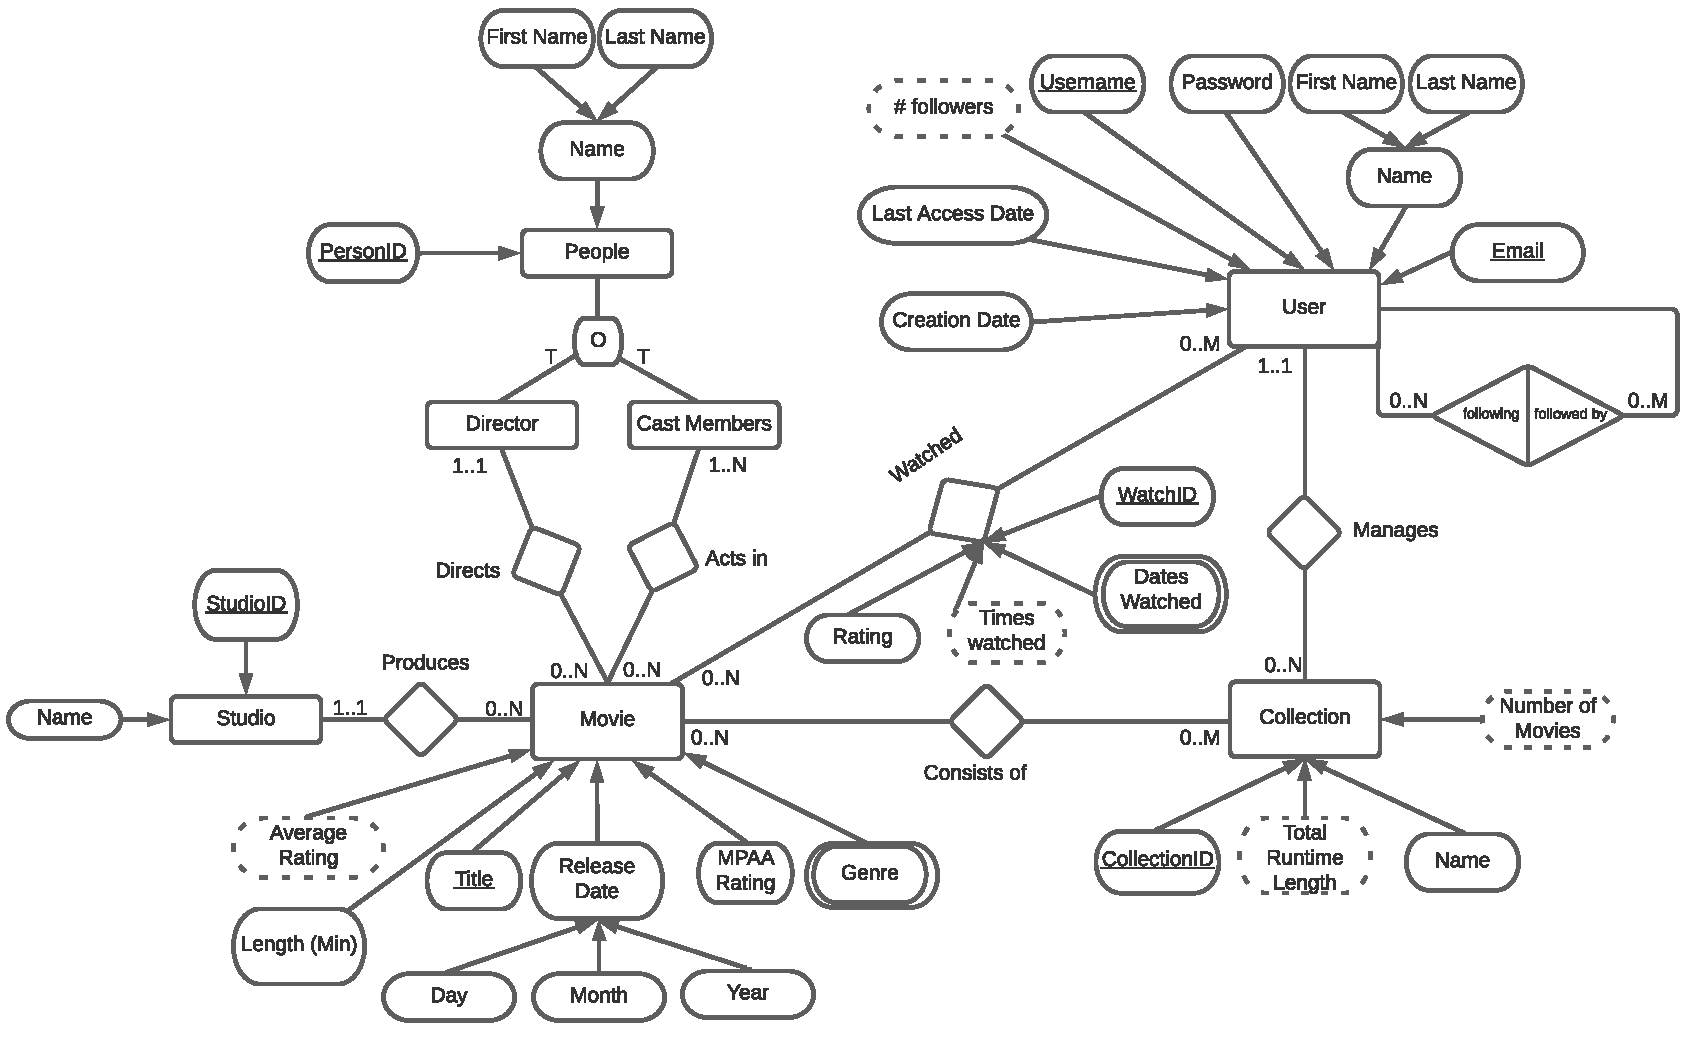
\includegraphics[scale=0.5]{images/Movies EER diagram.pdf}
                \label{EER Label}
                \caption {EER Diagram}
            \end{center}
        \end{figure}
    \end{landscape}


    Figure 1, seen above, is a conceptual data model of the database that will support the data and program requirements outlined in Section 1. In this section we provide a brief description of the entity, but primarily focus on the assumptions and design choices around the data model. Further descriptions about the attributes and entities can be found in Section 2.2: Reduction to tables, and data requirements can also be found in more detail in Section 2.3.

    \textbf{Users:} \\ The User entity represents one client’s account within the database. Two major relationships that User entities have to other entities include the Collection and Movie entities, where they track the user’s collections and individual movies watched respectively. Some of our design choices include that only one user can ever create a collection, but that a user can create zero or multiple collections, which necessitates a 1:N cardinality, and is a partial participation.
    As it relates to the Movie table, the idea behind this relationship is that we can have any number of users watch any number of movies, so the relationship between these tables should naturally be a N:M cardinality. Note that this requires separate tables when translating to the logical model, but this is described more in Section 2.2.
    Lastly, we have also defined a friend to be someone whom a user is currently following, and being followed by, another user. However, this is distinct from followers, where any one person can follow another - but the mere action of following that user does not indicate friendship. Since we want to support any number of individual users following any number of other users, and be able to be followed by any number of users, we have another N:M cardinality to indicate this relationship. \\ \\
    \textbf{Collections:} \\ The Collections entity represents the playlists of movies that a given user can have stored in their account. A given user can have 0 or more collections stored at a time, thus being 1:N cardinality, and can manage their collections via creating and naming a new collection (with no movies in it), deleting an existing collection, and adding or deleting movies from any of their collections. There is also a N:M cardinality between movies and collections, because any one movie should not be limited to a singular collection, and any one collection should naturally not be limited to a singular movie. \\ \\ \\
    \textbf{Movies:} \\ The Movies entity is the core of the product. It has a variety of relationships with other entities, many of which are described in their respective sections, but a brief description of the logic will be provided here.
    We are operating under the assumption that only a singular studio can produce a movie, but that a studio can produce zero or more movies. As a result, the relationship between Studio and Movies has a cardinality of 1:N. It should be noted that a movie must have a studio, so this is total participation.
    There is also a relationship between Movies and Directors, where we are similarly assuming that a singular director can direct a movie’s production, but that a single director can direct zero or more movies. Using this assumption, we have established the cardinality to be a 1:N relationship. It should be noted that a movie must have a director, so this is total participation.
    Cast members are an exception to this trend; while they are also in the total participation category, we are assuming that there must be at least one cast member to make a movie, but there can be more than one as well. There are no restrictions on the number of movies on which a cast member can work, so they can be involved in anywhere from 0 to many movies inclusive. This creates a N:M cardinality between these entities.
    Lastly, with regards to the collections, there can be zero or more movies in a collection, and zero or more collections can have any one movie. Assuming that this non-distinct membership requirement is in place, this would create an N:M cardinality as well.\\ \\
    \textbf{People:} \\ The People entity is related to 0 or more movies, and it has specialization to the Director Entity and Cast\textunderscore Member Entity. This specialization is overlapping and total as one person can be both a director and a cast member. The relationship between Director and Movies is 1:N (1..1 - 0..N) as every Movie needs exactly 1 director, while a director can direct 0 or more movies. The relationship between the Cast\textunderscore Member and Movies is N:M (1..N - 0..M) as a Movie must have at least 1 actor who acts in it while a cast member can act in 0 or more movies. We are assuming that every person has a first and last name and their id will be handled incrementally behind the scenes. \\ \\
    \textbf{Studio:} \\ The Studio entity describes both the name and unique ID of a movie studio, with each studio in the database relating to the Movie entity via having each studio produce 0..N movies in the database, thus being of 1:N cardinality. A assume that each studio must provide a name, and their id will be handled automatically by the database.

    \subsection{Reduction to tables}
    Collection(\underline{collectionID}, \emph{\underline{username}} (foreign), Name) \\
    Movie\textunderscore Collection(\emph{\underline{collectionID}} (foreign), \emph{title} (foreign)) \\
    User(\underline{Username}, password, first\textunderscore name, last\textunderscore name, email, last\textunderscore access, creation\textunderscore date, creation\textunderscore time)\\
    Following(\underline{\emph{follower\textunderscore username}}(foreign), \underline{\emph{followee\textunderscore username}}(foreign))\\
    User\textunderscore Movie(\underline{watchID}, \emph{\underline{username}} (foreign), \emph{\underline{title}} (foreign), rating)\\
    Dates\textunderscore Watched(\emph{\underline{watchID}} (foreign), date)\\
    Studio (\underline{StudioID}, Name)\\
    Movie(\underline{Title}, length, release\textunderscore date, MPAA\textunderscore rating)\\
    Movie\textunderscore Cast\textunderscore Member(\emph{\underline{Title}} (foreign), \emph{\underline{personID}} (foreign)) \\
    People(\underline{personID}, first\textunderscore name, last\textunderscore name)\\
    Director(\underline{\emph{personID}}(foreign))\\
    Cast\textunderscore Member(\emph{\underline{personID}} (foreign))\\
    Genre(\underline{GenreID}, \emph{\underline{Title}} (foreign))\\
    Movie\textunderscore Director(\emph{\underline{Title}} (foreign), \emph{\underline{directorID}} (foreign)) \\
    Studio\textunderscore Movie(\underline{\emph{studio\textunderscore id}}(foreign), \underline{\emph {title}}(foreign)

    \textbf{User:} The user entity’s attributes are mostly directly related to the user and are not needed within any of the other entities, so these attributes are mostly singular. This includes the username, password, email, last access date, and creation date - which are all singular attributes that compose their own columns. The one exception is the name attribute, which is a composite attribute, which was translated to the table by making separate columns for the first name and last name attributes. There is one derived attribute, number of followers, which will be derived by counting all of the rows in the Following table where the followee\textunderscore username is the current user’s username. \\ \\
    \textbf{Following:} The Following table was created because of the N:M mapping with the “following/followed by” relationship, this relationship constitutes its own table where we can store two user’s usernames in a row, where the first is the follower, and the second is the followee. This enables any one user to have multiple followers and follow multiple people without having redundant data in the User table. \\ \\
    \textbf{Collection:} This table represents a collection of movies that a user can build, and only has two simple attributes that are directly implemented as columns: collectionID and name. However, the information regarding what movie is in a collection is stored in another table because each table needs to support multiple movies - a requirement that we couldn't easily achieve by including movies within this Collection table. Therefore, this additional Movie\textunderscore Collection table, described in more detail below, was made to accommodate each movie in a collection. There are two derived attributes associated with this table, one of which is total runtime - which can be derived by summing the runtime of each movie within the collection - and number of movies, which can be derived by counting the number of distinct titles within each collection. \\ \\
    \textbf{Movie\textunderscore Collection:} This table records all the movies that are entered into a user's collection by holding the collectionID with which that row is associated, and the title of the movie. This decomposition was necessary because each collection needs to be able to store multiple movies, so by having this decomposition we can easily search for all movies in a collection by using the collectionID. \\ \\
    \textbf{User\textunderscore Movie:} This table is a necessary decomposition because of the N:M relationship between the User and Movie entities. This table maintains a history of which user has watched which movie, and must include the username and title of the user and movie respectively in order to uniquely identify a tuple. Other attributes such as the times watched and rating from that user are also recorded so that we can support popularity gauges by customers, where times watched is derived and can be determined by counting the number of times a given username and movieID appear in the table.\\ \\
    \textbf{Dates\textunderscore Watched:} This includes a watchID to uniquely identify the dates on which a user watched a particular movie, which is recorded in order to accurately gauge popularity of content. This is a separate table from the User\textunderscore Movie because a movie can be watched repeatedly, and is therefore inherently multivalued. Using the watchID as a foreign key, we can uniquely record when a user watches a particular movie.\\ \\
    \textbf{Studio:} This table is necessary because of the 1:N relationship studios have with movies. By having a separate table it ensures that a single studio can be responsible for many movies, but a movie will always have a studio. Furthermore a separate studio table ensures that each studio can be uniquely identified by an ID number and there are no anomalies when deleting movies - namely, deletion anomalies that would remove a studio from the database if the movie that a studio produced was deleted.\\ \\
    \textbf{Movie:} This table This entity records the details of a movie in the database. It has many simple attributes like title, length, release date, as well as the MPAA rating. Other attributes that identify the studio and director must also be included so that we can uniquely identify them, and also to prevent deletion anomalies that remove these entities from the database if the movie was ever removed. There is also an average rating attribute that can be derived by finding all of the ratings correlated with that movie title in the User\textunderscore Movie table and dividing by the total number of ratings to yield an average.\\ \\
    \textbf{Movie\textunderscore Cast\textunderscore Member:} Since there is a N:M relationship between movies and cast members, we created a separate table to record which movies a cast member appears in by recording the movie title and the cast member's ID. In this way a cast member can work on multiple movies and a movie can have multiple cast members.\\ \\
    \textbf{People:} This table is one where it assigns a person an ID number and provides a first and last name. This table's purpose is to be a superclass for the specializations of Director and Cast Member, which have common attributes. The relationship is total and overlapping, meaning that a someone cannot be a "Person", they must be either a director or a cast member, or possibly both.\\ \\
    \textbf{Director:} This table is responsible for nothing more than identifying which Person objects are contained within the directors specialization for a movie, so that they can be entered into the movie entity\\ \\
    \textbf{Cast\textunderscore Member:} Much like the director table, this table is merely a declarator for the Cast Member specialization. It identifies a person as a cast member so that they can be added to a movie entity.\\ \\
    \textbf{Genre:} The genre table is necessary because a movie can have more than one genre instead of simply one genre, so because of the multivalued nature of the attribute we specified a new table where each row holds the movie Title, the GenreID, and the GenreName. This enables multiple genres to be stored for one movie, and accessible by its title.\\

    \subsection{Data Requirements/Constraints}
    \textbf{Not Null Attributes:}\\
    \textbf{Collection:} Name\\
    \textbf{User:} Password, first\textunderscore name, last\textunderscore name, email, last\textunderscore access, creation\textunderscore date\\
    \textbf{Dates\textunderscore Watched:} Date\\
    \textbf{Studio:} Name\\
    \textbf{Movie:} Length, Release\textunderscore date, MPAA\textunderscore rating, studio\textunderscore id, director\textunderscore id\\
    \textbf{People:} first\textunderscore name, last\textunderscore name\\
    \textbf{Genre:} Genre\textunderscore name

    \subsection{Sample instance data}
    \textbf{Collection Ex:}\\
    1.(\underline{1}, \emph{\underline{user1}}, MyMovies)\\
    2.(\underline{2}, \emph{\underline{user2}}, SadMovies)\\
    3.(\underline{3}, \emph{\underline{user3}}, HappyMovies)\\
    4.(\underline{4}, \emph{\underline{user4}}, LongMovies)\\
    5.(\underline{5}, \emph{\underline{user5}}, ShortMovies)\\
    \\ \\
    \textbf{Movie}\textunderscore Collection Ex:\\
    1.(\underline{\emph{1}},\underline{\emph{2}})\\
    2.(\underline{\emph{2}},\underline{\emph{4}})\\
    3.(\underline{\emph{3}},\underline{\emph{6}})\\
    4.(\underline{\emph{4}},\underline{\emph{8}})\\
    5.(\underline{\emph{5}},\underline{\emph{10}})\\
    \\ \\
    \textbf{User Ex:}\\
    1. (\underline{greg303}, password1, Greg, Lee, greg@gmail.com, 2021-5-1, 2014-1-1)\\
    2. (\underline{george204}, password2, George, Martin, martin-is-amazing@gmail.com, 2020-1-5,2014-6-12)\\
    3. (\underline{avery939}, password3, Avery, Clark, avery939@gmail.com, 2021-7-5, 2014-5-7)\\
    4. (\underline{coolkid503}, password4, Carlos, Perez, cool-kid503@gmail.com, 2022-12-5, 2014-4-4)\\
    5. (\underline{victor118}, password5, Victor, Metic, victor118@gmail.com, 2021-10-23, 2016-6-6) \\
    \\ \\
    \textbf{Following:}\\
    1. (\emph{\underline{freddie1}}, \emph{\underline{maddie1}})\\
    2. (\emph{\underline{carson1}}, \emph{\underline{shannon1}})\\
    3. (\emph{\underline{ben1}}, \emph{\underline{emily1}})\\
    4. (\emph{\underline{peter1}}, \emph{\underline{tobias2}})\\
    5. (\emph{\underline{harry1}}, \emph{\underline{simon1}})\\
    \\ \\
    \textbf{User\textunderscore Movie Ex:}\\
    1.(\underline{1}, \underline{\emph{user1}}, \underline{\emph{Megamind}}, 4)\\
    2.(\underline{2}, \underline{\emph{user2}}, \underline{\emph{Jaws}}, 4)\\
    3.(\underline{3}, \underline{\emph{user3}}, \underline{\emph{Jaws 2}}, 4)\\
    4.(\underline{4}, \underline{\emph{user4}}, \underline{\emph{Finding Nemo}}, 4)\\
    5.(\underline{5}, \underline{\emph{user5}}, \underline{\emph{Finding Dory}}, 4)\\
    \\ \\
    \textbf{Dates\textunderscore Watched Ex:}\\
    1. (\emph{\underline{0213}}, 2021-14-5)\\
    2. (\emph{\underline{0213}}, 2021-3-12)\\
    3. (\emph{\underline{0213}}, 2020-6-20)\\
    4. (\emph{\underline{0213}}, 2021-3-4)\\
    5. (\emph{\underline{0213}}, 2015-10-19)\\
    \\ \\
    \textbf{Studio Ex:}\\
    1. (\underline{1}, Dreamworks)\\
    2. (\underline{2}, Disney)\\
    3. (\underline{3}, Universal)\\
    4. (\underline{4}, Warner Bros)\\
    5. (\underline{5}, MGM)\\
    \\ \\
    \textbf{Movie Ex:}\\
    1.(\underline{Megamind}, 96, 2010-10-30, PG, \emph{1},\emph{0006})\\
    2.(\underline{Lord of the Rings}, 2001-12-19, \emph{2}, \emph{0007})\\
    3.(\underline{Finding Nemo}, 120, 2003-05-30, \emph{1}, \emph{0008})\\
    4.(\underline{Jaws}, 150, 1975-6-20, \emph{3},\emph{0009})\\
    5.(\underline{Jurassic Park}, 120, 1993-6-11, \emph{4}, \emph{0010})\\
    \\ \\
    \textbf{Movie\textunderscore Cast\textunderscore Member Ex:}\\
    1. (\underline{Star Wars}, \emph{0007})\\
    2. (\underline{Avengers}, \emph{0008})\\
    3. (\underline{Coco}, \emph{0003})\\
    4. (\underline{Ghostbusters}, \emph{0015})\\
    5. (\underline{Avatar}, \emph{0019})\\
    \\ \\
    \textbf{People Ex:}\\
    1. (\underline{0006}, Tom, McGrath)\\
    2. (\underline{0007}, James, Cameron)\\
    3. (\underline{0008}, Steven, Spielberg)\\
    4. (\underline{0009}, Christopher, Nolan)\\
    5. (\underline{0010}, Peter, Jackson)\\
    \\ \\
    \textbf{Director Ex:}\\
    1. (\underline{\emph{0006}})\\
    2. (\underline{\emph{0007}})\\
    3. (\underline{\emph{0008}})\\
    4. (\underline{\emph{0009}})\\
    5. (\underline{\emph{0010}})\\
    \\ \\
    \textbf{Cast\textunderscore Member Ex:} \\
    1. (\underline{\emph{0001}})\\
    2. (\underline{\emph{0002}})\\
    3. (\underline{\emph{0003}})\\
    4. (\underline{\emph{0004}})\\
    5. (\underline{\emph{0005}})\\
    \\ \\
    \textbf{Genre Ex}:\\
    1. (\underline{1}, \emph{\underline{Husk}})\\
    2. (\underline{2}, \emph{\underline{Lord of the Rings}})\\
    3. (\underline{3}, \emph{\underline{Up}})\\
    4. (\underline{4}, \emph{\underline{Spiderman}})\\
    5. (\underline{5}, \emph{\underline{Titanic}})\\
    \\ \\


    \section{Implementation}
    \textbf{Sample Table Creation SQL}\\ \\
    Create table p320\textunderscore 02.User
    (username varchar(20) primary key, \\
    password varchar(20) not null,\\
    first\textunderscore name varchar(20) not null,\\
    last\textunderscore name varchar(20) not null,\\
    email varchar(30) not null,\\
    last\textunderscore access date not null,\\
    creation\textunderscore date date not null,\\
    constraint unique\textunderscore email\textunderscore user unique(email))\\ \\


    \noindent Create table p320\textunderscore 02.Movie\textunderscore Collection\\
    (collection\textunderscore ID int,\\
    title varchar(50),\\
    primary key (collection\textunderscore ID, title),\\
    foreign key(collection\textunderscore ID) references Collection(collection\textunderscore ID) on delete cascade on update cascade,\\
    foreign key(title) references Movie(title) on delete cascade on update cascade)\\ \\

    \noindent\textbf{Sample Table Population SQL} \\ \\
    \noindent Table: cast\textunderscore member \\
    insert into p320\textunderscore02.cast\textunderscore member(person\textunderscore id)
    values (14441)\\
    insert into p320\textunderscore02.cast\textunderscore member(person\textunderscore id)
    values (14442)\\

    \noindent Table: collection \\
    insert into p320\textunderscore02.collection(username, name)
    values ('mjh9122', 'myMovies')\\
    insert into p320\textunderscore02.collection(username, name)
    values ('bob123', 'sadMovies')\\

    \noindent Table: director \\
    insert into p320\textunderscore02.director(person\textunderscore id)
    values (14441)\\
    insert into p320\textunderscore02.director(person\textunderscore id)
    values (14442)\\

    \noindent Table: following \\
    insert into p320\textunderscore02.following(following\textunderscore username, followee\textunderscore username) \\
    values ('dmc1542', 'mjh9122')\\ \\
    insert into p320\textunderscore02.following(following\textunderscore username, followee\textunderscore username) \\
    values ('dmc1542', 'mjh9122')\\

    \noindent Table: genre \\
    insert into p320\textunderscore02.genre(name) values ('action')\\
    insert into p320\textunderscore02.genre(name) values ('adventure')\\

    \noindent Table: genre\textunderscore movie \\
    insert into p320\textunderscore02.genre\textunderscore movie(genre\textunderscore id, title) values (2, 'Shrek')\\
    insert into p320\textunderscore02.genre\textunderscore movie(genre\textunderscore id, title) values (3, '1917')\\

    \noindent Table: movie \\
    insert into p320\textunderscore02.movie(title, length, release\textunderscore date, mpaa\textunderscore rating)\\
    values ('Logan', 137, '2017-05-16', 'R') \\ \\
    insert into p320\textunderscore02.movie(title, length, release\textunderscore date, mpaa\textunderscore rating)\\
    values ('Amy',128, '2016-07-27, 'R')\\ \\

    \noindent Table: movie\textunderscore cast \textunderscore member\\
    insert into p320\textunderscore02.movie\textunderscore cast \textunderscore member(title, person\textunderscore id) values ('Shrek', 10000)\\
    insert into p320\textunderscore02.movie\textunderscore cast \textunderscore member(title, person\textunderscore id) values ('Shrek', 12983)\\

    \noindent Table: movie\textunderscore collection\\
    insert into p320\textunderscore02.movie\textunderscore collection(collection\textunderscore id, title) values (5, 'Logan')\\
    insert into p320\textunderscore02.movie\textunderscore collection(collection\textunderscore id, title) values (5, 'Amy")\\

    \noindent Table: movie\textunderscore director\\
    insert into p320\textunderscore02.movie\textunderscore director(title, director\textunderscore id) values ('Shrek', 18773)\\
    insert into p320\textunderscore02.movie\textunderscore director(title, director\textunderscore id) values ('Shrek 2', 18773)\\

    \noindent Table: person\\
    insert into p320\textunderscore02.person(first\textunderscore name, last\textunderscore name) values ('Michael', 'Bay')\\
    insert into p320\textunderscore02.person(first\textunderscore name, last\textunderscore name) values ('Agi', 'Orsi')\\

    \noindent Table: studio\textunderscore movie\\
    insert into p320\textunderscore02.studio\textunderscore movie(studio\textunderscore id, title) values (9, 'Logan')\\
    insert into p320\textunderscore02.studio\textunderscore movie(studio\textunderscore id, title) values (220, 'Logan')\\

    \noindent Table: user\\
    insert into p320\textunderscore02.user \\(username, password, first\textunderscore name, last\textunderscore name, email, last\textunderscore access, creation\textunderscore date) \\
    values \\ ('mjh9122', 'password', 'Michael', 'Holtz', 'mjh9122@rit.edu', '2022-03-17', '2022-03-17')\\ \\
    insert into p320\textunderscore02.user \\(username, password, first\textunderscore name, last\textunderscore name, email, last\textunderscore access, creation\textunderscore date) \\
    values \\('dmc1542', 'password', 'Domenic', 'Cacace', 'dmc1542@rit.edu', '2022-03-17', '2022-03-17')\\

    \noindent Table: user\textunderscore movie\\
    insert into p320\textunderscore02.user\textunderscore movie(username, title, last\textunderscore watched, rating)\\ values ('mjh9122', 'Logan', '2022-03-17', 4)\\
    insert into p320\textunderscore02.user\textunderscore movie(username, title, last\textunderscore watched, rating)\\ values ('mjh9122', 'Amy', '2022-03-17', 2)\\

    In order to load values into our database we started with a rotten tomatoes database that contained all of the information necessary for the project and more. We then extracted the columns that we needed and loaded them into a temporary data table in our data base. We needed to convert some data types in order to have them mesh with our existing tables. One example of this was converting the length of a movie from a string with hours and minutes to an integer that only represents minutes. Another problem that we ran into while loading the data was compiling a list of all actors and all directors as they were stored in comma separated lists for each movie in our temporary data file. In order to make these lists, Domenic was able to write scripts that generated csv files with every unique actor and director, these scripts, that we later applied to studio and genre as well, were integral to our data loading process. Once we had all of the entity type tables populated, we moved on to the relationship type tables. We then leaned even more heavily on Domenic's scripts to populate those tables, with these new programs calling SQL queries to identify all of the needed tuples to populate tables such as movie\textunderscore cast \textunderscore member, movie\textunderscore collection, movie\textunderscore director, and genre\textunderscore movie.


    \section{Data Analysis}

    \subsection{Hypothesis}
    Use this section to state the objectives of your data analysis; what are the observations you are expecting to find. Note that your final
    observations may end up differing from your proposal, that is also a valid result.

    \subsection{Data Preprocessing}
    Use this section to describe the preprocessing steps you have performed to prepare the data for the analytics. Preprocessing steps may include: data cleaning (e.g., filling missing values, fixing outliers), formatting the data (e.g., resolving issues like inconsistent abbreviations, multiples date format in the data), combining or splitting fields, add new information (data enrichment).

    Explain how the data was extracted from the database for the analysis; if you used complex queries or views, or both.

    \subsection{Data Analytics \& Visualization}
    Use this section to explain the process/techniques used to analyze the data, use data visualization to present the results, and explain them.

    \subsection{Conclusions}
    Use this section to explain the conclusions drawn from your data analysis.\\


    \section{Lessons Learned}
    In Phase 1 of the development of the project, we had originally planned on the creation of a chat feature that would allow users to chat with their friends while watching movies in order to enhance the moviegoing experience and increase the social interaction possible on the platform. However, by Phase 2 of the project, we had made the decision to completely remove this feature from the overall design while in the process of creating the EER diagram after deciding that the product delivered to the customer should primarily focus on the minimum functionality. It is more important to G2 Software to deliver a Minimum Viable Product (MVP) and prioritize our efforts on creating a bug-free experience.\\

    {\bf The next subsection is meant to provide you with some help in
    dealing with figures, tables and references, as these are sometimes
    hard for folks new to \LaTeX. Your figures and tables
    may be distributed all over your paper (not just here), as appropriate for your paper.

    Please delete the following subsection before you make any submissions!}

    \subsection{Tables, Figures, and Citations/References}

    Tables, figures, and references in technical
    documents need to be presented correctly. As many students
    are not familiar with using these objects, here is a quick
    guide extracted from the ACM style guide.

    \begin{table}
        \centering
        \caption{Feelings about Issues}
        \label{SAMPLE TABLE}
        \begin{tabular}{|l|r|l|}
            \hline
            Flavor  & Percentage & Comments              \\ \hline
            Issue 1 & 10\%       & Loved it a lot        \\ \hline
            Issue 2 & 20\%       & Disliked it immensely \\ \hline
            Issue 3 & 30\%       & Didn't care one bit   \\ \hline
            Issue 4 & 40\%       & Duh?                  \\ \hline
        \end{tabular}
    \end{table}


    First, note that figures in the report must be original, that is,
    created by the student: please do not cut-and-paste figures from any
    other paper or report you have read or website. Second, if you do need to include figures,
    they should be handled as demonstrated here. State that
    Figure~\ref{SAMPLE FIGURE} is a simple illustration used in the ACM
    Style sample document. Never refer to the figure below (or above)
    because figures may be placed by \LaTeX{} at any appropriate location
    that can change when you recompile your source $.tex$
    file. Incidentally, in proper technical writing (for reasons beyond
    the scope of this discussion), table captions are above the table and
    figure captions are below the figure. So the truly junk information
    about flavors is shown in Table~\ref{SAMPLE TABLE}.


    \section{Resources}
    Include in this section the resources you have used in your project beyond the normal code development such as data sets or data analytic tools (i.e. Weka, R).
\end{document}

